\chapter{Connected Evidence Selection for Language Models with AGRAG}
\label{ch:agrag}

This chapter is based on \emph{AGRAG: Advanced Graph-based Retrieval-Augmented Generation for LLMs}, published at ICDE 2026~\cite{agrag-paper}. It studies how a retrieval system can select connected evidence and communicate the relationships among retrieved facts to a language model. The task extends beyond retrieving a relevant label. An answer may require several facts, their connections, and the surrounding passages that explain them.

\section{Research Problem and Evidence Requirements}
\label{sec:agrag:problem}
A retrieval system can locate passages relevant to a question while still leave the generator with the task of discovering how those passages fit together. This distinction matters when a question asks for a summary, an explanation, or a response that combines information from different parts of a corpus. Similar passages may repeat one fact. Passages containing different parts of an answer may share few words. A graph provides an explicit representation of these connections, but the system must still decide which part of the graph to supply to the generator.

The research question in this chapter is how to select evidence that combines query relevance with connectivity. There are two related decisions. The first concerns the construction of the graph from text. Extracted entities establish the vocabulary over which subsequent retrieval operates. The second concerns the subgraph returned for a query. A ranking of individual nodes assigns relevance scores, whereas a connected subgraph also specifies relationships among the selected items. AGRAG addresses these decisions through statistical entity extraction, influence-aware graph retrieval, and a separate hybrid passage retrieval channel.

Consider a corpus containing statements about an illness, the organ that it affects, and the routes through which it spreads. A query may match facts mentioning the illness and the organ. Connecting those facts can identify a small initial structure, but answering the question may require a neighboring fact that specifies another anatomical component. The original example in Figure~\ref{fig:agrag:example} illustrates this distinction. The example motivates expansion beyond an initial terminal-connecting structure. It is a qualitative account of evidence selection; quantitative evaluation is provided separately in Section~\ref{sec:agrag:experiments}.

The input is a text corpus $\mathcal{T}$ and a natural-language query $q$. The corpus is divided into chunks $\mathcal{T}_c$. The indexed graph $\mathcal{G}=(\mathcal{V},\mathcal{E})$ contains entity nodes, passage nodes, and several kinds of edges. Query processing identifies an initial set of relevant triple facts, assigns node influence scores and edge costs, and produces a subgraph for generation. A hybrid retriever supplies additional passages from the same corpus. The output is an answer conditioned on the query, a textual serialization of the retrieved graph, and the hybrid passages.

The evidence representation has two levels. Entity and relation information expresses specific connections. Passage nodes preserve links to the text from which those connections were extracted. The graph serialization gives the generator a relational account of the retrieved material, while passages provide the language surrounding those facts. This division is central to AGRAG. A retrieved graph may identify the relevant relationship without preserving every qualification or explanatory detail in a paragraph. The hybrid channel supplies contextual material alongside the graph.

The chapter evaluates the resulting pipeline on tasks with different answer requirements. Fact retrieval emphasizes individual facts. Complex reasoning combines facts. Contextual summarization requires coverage of several evidence items. Creative generation evaluates responses grounded in retrieved material while allowing more flexible output. Text classification supplies a further setting in which graph retrieval identifies candidate labels. Each task retains its own evaluation protocol, so the results are interpreted by task rather than combined into a single measure of reasoning.

\section{Framework and Graph Construction}
\label{sec:agrag:construction}
\subsection{The three-stage pipeline}
AGRAG separates data preparation, graph retrieval, and hybrid retrieval. Data preparation builds the graph and the passage indexes. Graph retrieval conditions the graph on a query through semantic mapping and influence scores, then selects a connected evidence subgraph. Hybrid retrieval combines dense passage similarity with BM25. Figure~\ref{fig:agrag:pipeline} reproduces the original architecture.

\begin{figure}[tbp]
\centering
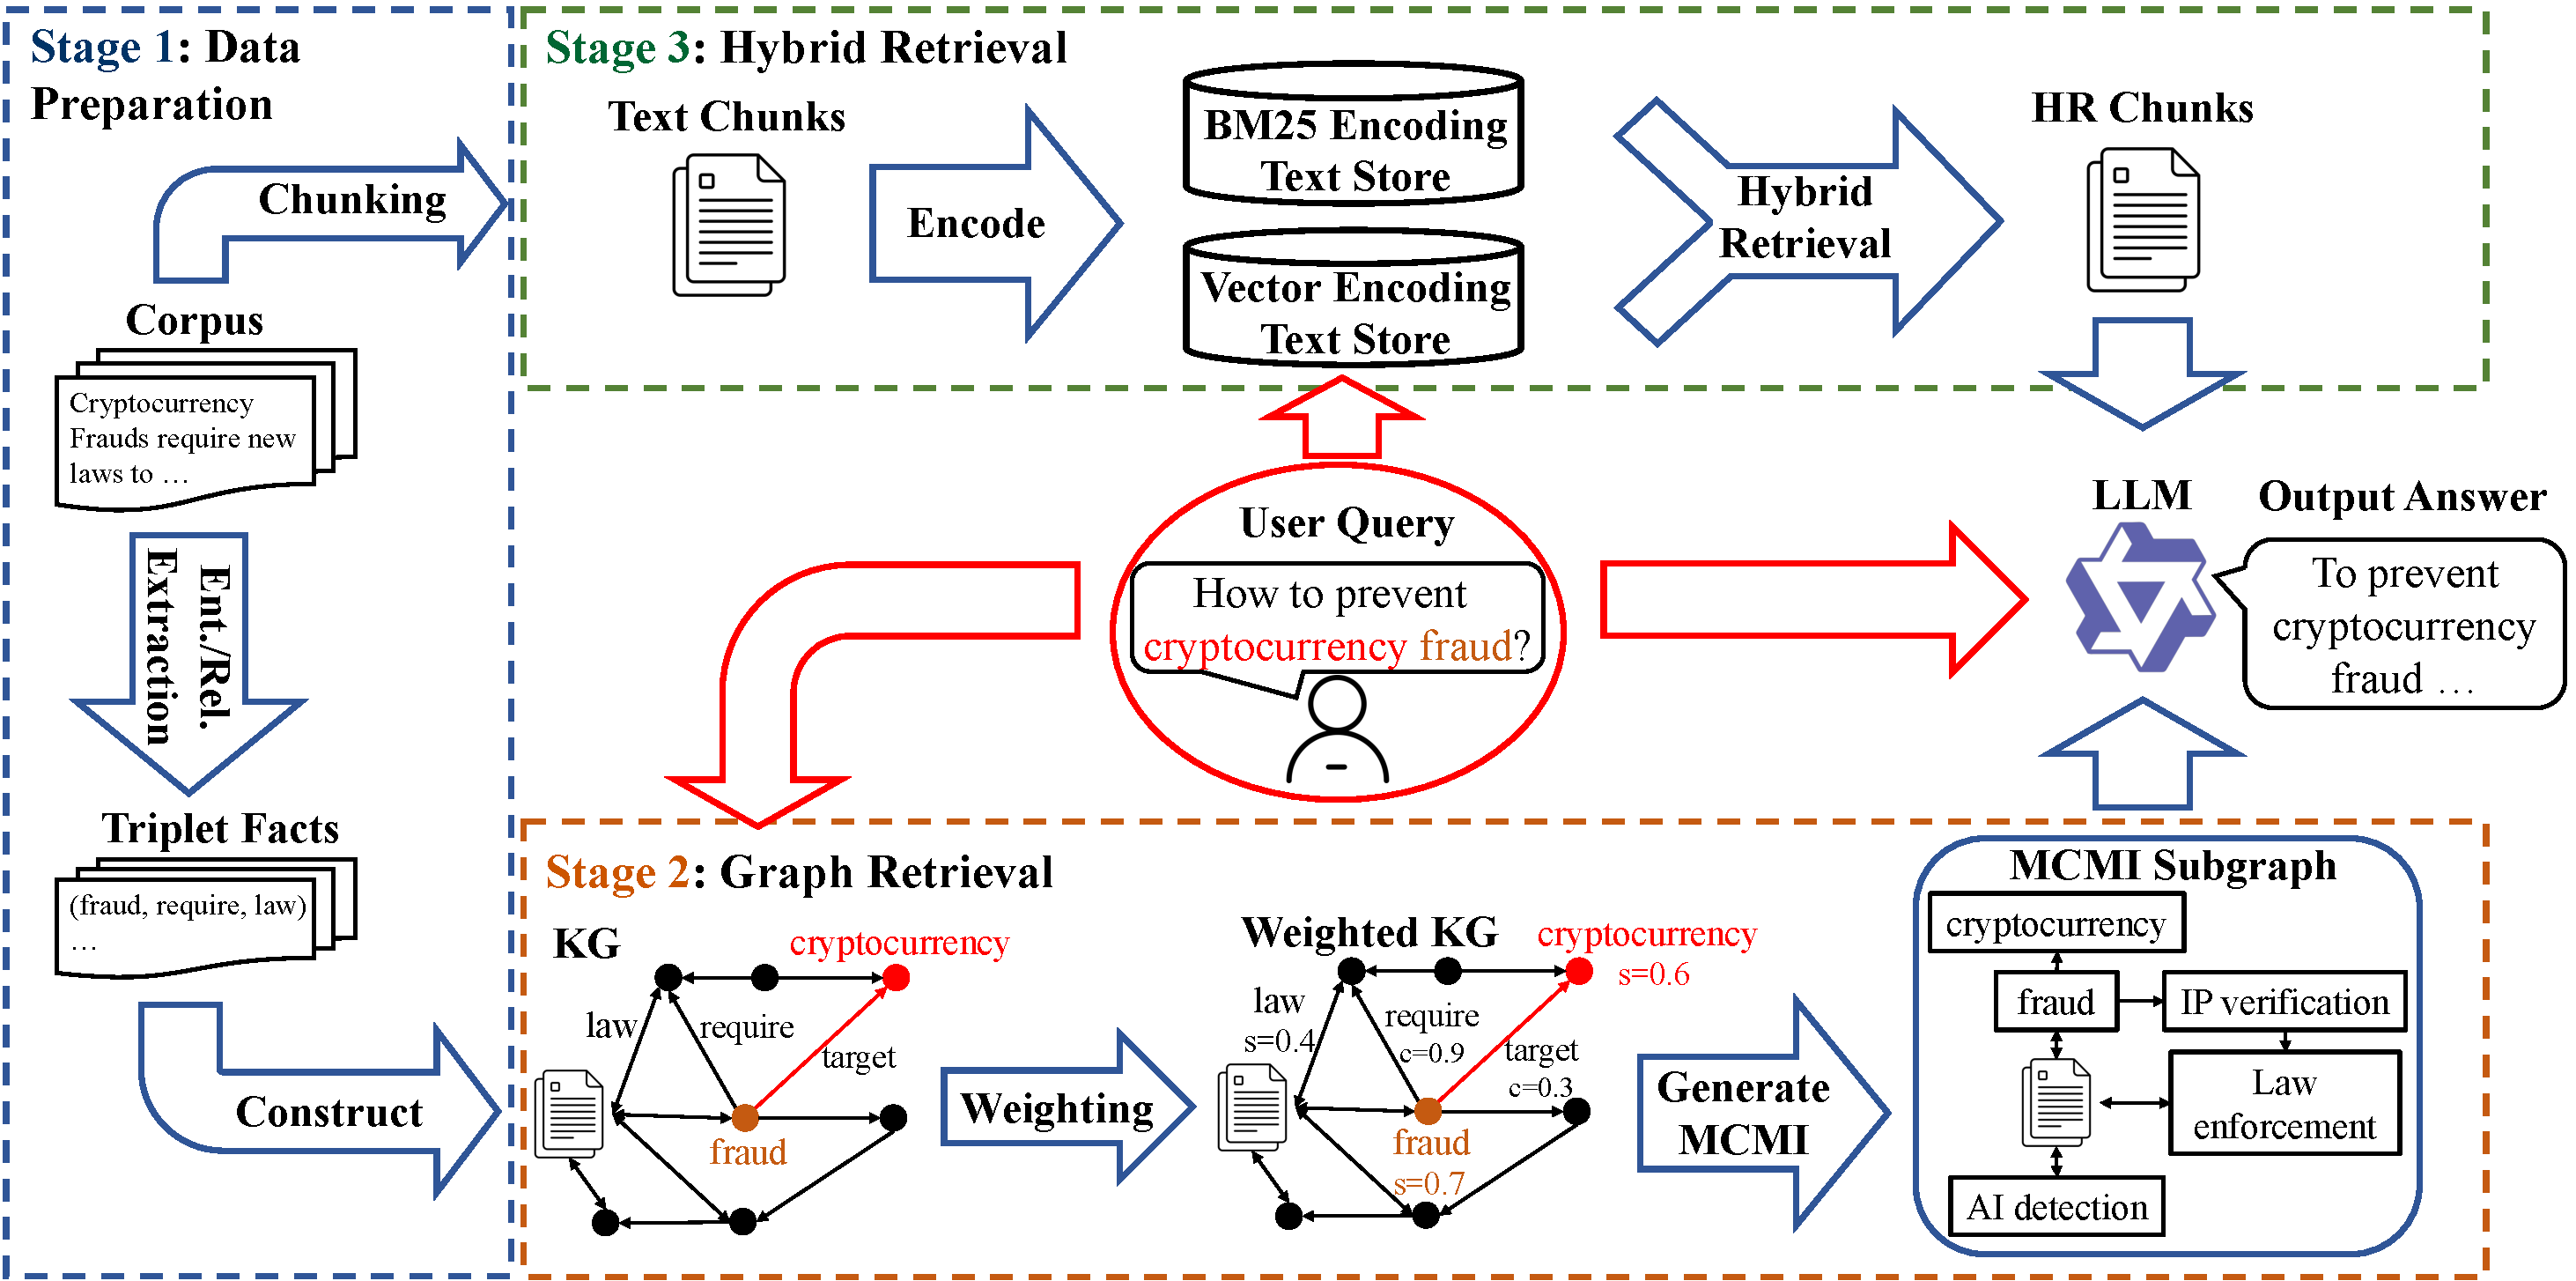
\includegraphics[width=\textwidth]{figures/agrag/AGRAG_pipeline.pdf}
\caption{The AGRAG pipeline. The original figure separates corpus preparation, query-conditioned graph retrieval, and hybrid passage retrieval. Reproduced from Figure 1 of the source paper~\cite{agrag-paper}.}
\label{fig:agrag:pipeline}
\end{figure}

The stages have different update requirements. Chunking, entity extraction, relation extraction, and the construction of passage links belong to corpus indexing. Mapping a query to graph facts, computing its influence scores, and expanding its evidence subgraph occur during query processing. Dense and sparse passage indexes support the hybrid channel. This organization identifies which costs arise from preparing the corpus and which recur for each query.

The statistical component replaces the entity extraction step used in the compared graph pipelines. Language models remain involved in relation extraction, filtering raw mapped triples, and generating answers. The distinction between these roles is necessary for understanding both the method and its ablation. Replacing entity extraction changes the nodes provided to later stages; it does not remove every model-generated component from the graph.

\subsection{Chunking and statistical entity extraction}
The corpus is split into overlapping text chunks,
\begin{equation}
\mathcal{T}_c=\operatorname{Split}(\mathcal{T},l_t,l_o),
\label{eq:agrag:chunking}
\end{equation}
where $l_t$ is the chunk length and $l_o$ is the overlap. The reported main setting uses 256 tokens per chunk and an overlap of 32 tokens. Overlap allows adjacent chunks to share text at their boundaries; the graph subsequently connects chunks through the entities they contain.

AGRAG considers words and phrases up to a maximum n-gram length $b$. For a candidate term $v$ in chunk $t$, the source defines the extraction score
\begin{equation}
\operatorname{ER}(v,t)=
\frac{\operatorname{count}(v,t)}{|t|\log(|\mathcal{T}_c|+1)}
\log\frac{|\mathcal{T}_c|+1}{|\{t_j\in\mathcal{T}_c:v\in t_j\}|+1}.
\label{eq:agrag:extraction-score}
\end{equation}
The first factor depends on within-chunk frequency and length. The second distinguishes terms according to their distribution across chunks. The extracted set is
\begin{equation}
\mathcal{V}_t=\{v:\operatorname{ER}(v,t)>\tau\},
\label{eq:agrag:entities}
\end{equation}
with maximum n-gram length $b$ and threshold $\tau$ controlling candidate boundaries and selection. The main paper reports $b=3$ and $\tau=0.5$. Equations~\ref{eq:agrag:extraction-score}--\ref{eq:agrag:entities} preserve the source formulation.

The extraction rule uses terms appearing in the corpus. This constrains the origin of entity strings and makes their relationship to the indexed text explicit. Its decisions are based on term statistics, so linguistic salience and factual importance need not coincide. A frequently mentioned generic term and a rare but relevant phrase have different statistical profiles. The sensitivity experiment therefore examines both the phrase boundary and the extraction threshold.

An entity string identifies a graph node, while its occurrences connect that node to passages. This provides a path from fine-grained graph retrieval back to textual evidence. A shared entity can also connect information across chunks. The utility of these connections depends on whether the extracted string captures the intended entity and whether occurrences have compatible meanings. The evaluation measures the complete retrieval and generation pipeline under the reported extraction settings.

\subsection{Relations, passage nodes, and synonyms}
For each chunk, the language model receives the selected entity set and the chunk text, and extracts relations,
\begin{equation}
\mathcal{E}_t=\operatorname{LLM}(\mathcal{V}_t,t,p_{\mathrm{re}}).
\label{eq:agrag:relations}
\end{equation}
The prompt $p_{\mathrm{re}}$ asks for relations between the extracted entities in the chunk. The resulting entity--relation--entity triples provide the graph's factual edges. The statistical stage and the model stage therefore operate consecutively: one selects entity candidates from observed terms, and the other supplies relations conditioned on those candidates and their context.

Chunks are also inserted as passage nodes. A \textit{Contains} edge connects a passage to an entity extracted from it. These links preserve the association between the symbolic representation and the source chunk. They also allow paths to cross passages through shared entities. A passage contributes contextual evidence to graph retrieval without being reduced to a single isolated fact.

The graph includes synonym edges between entity nodes whose embedding similarity exceeds a threshold $\varphi$. Such an edge expresses an embedding-based correspondence between strings. It permits retrieval to connect different expressions that would otherwise form separate nodes. Its role differs from an extracted relation: an extracted relation comes from the language model's reading of a chunk, whereas a synonym edge comes from a similarity test. Both affect graph connectivity, and both remain part of the retrieval conditions.

AGRAG additionally introduces a pseudo node linked to passage nodes. The reported cost of each pseudo edge is 10. This connection gives the graph a route between otherwise disconnected portions while penalizing its use relative to semantically relevant factual edges. The pseudo connection is an indexing device, so it should be distinguished from a factual assertion in the source corpus when interpreting the retrieved structure.

\section{Query Mapping and Influence-aware Retrieval}
\label{sec:agrag:influence}
\subsection{Mapping a query to triple facts}
At query time, AGRAG first identifies facts that are semantically close to the query. A text encoder $\mathcal{M}$ maps the query and a textual rendering of each triple to vectors. With $\mathbf{q}=\mathcal{M}(q)$ and $\mathbf{f}=\mathcal{M}(f)$, the mapping score is
\begin{equation}
\operatorname{MS}(\mathbf{q},\mathbf{f})=
\cos(\mathbf{q},\mathbf{f}).
\label{eq:agrag:mapping}
\end{equation}
The highest-scoring $k_a$ facts form the raw mapped set $\mathcal{F}_{\mathrm{raw}}$. The main setting uses $k_a=5$. This stage locates candidate facts in the indexed graph before graph propagation begins.

A model-based filtering step then evaluates the raw facts with respect to the query,
\begin{equation}
\mathcal{F}=\operatorname{LLM}(\mathcal{F}_{\mathrm{raw}},q,p_{\mathrm{tf}}).
\label{eq:agrag:filter}
\end{equation}
The filtered set $\mathcal{F}$ defines the query anchors. Dense mapping and filtering play different roles. Dense mapping produces a short candidate list efficiently. Filtering evaluates the candidates jointly with the actual query. The filtering ablation removes the second operation and tests its contribution to answer quality and cost.

The anchors determine where graph retrieval starts. They do not themselves specify the complete answer context. Facts connecting or surrounding the mapped set can be useful even when their direct similarity to the query is lower. Graph influence provides a way to score these surrounding items using their connection to the mapped facts. Edge costs then retain a separate measure of semantic relevance during subgraph construction.

\subsection{Node influence and edge costs}
AGRAG uses a personalized PageRank-style propagation to assign query-dependent influence scores,
\begin{equation}
\mathbf{s}=\lim_{i\rightarrow\infty}\mathbf{s}^{(i)},\qquad
\mathbf{s}^{(i)}=(1-d)\mathbf{p}+d\mathbf{P}\mathbf{s}^{(i-1)}.
\label{eq:agrag:propagation}
\end{equation}
Here $\mathbf{p}$ is determined by nodes associated with the filtered mapped facts, and $\mathbf{P}$ is the graph propagation matrix specified in the source. The reported setting uses $d=0.5$ and stops the iteration when the change is below $10^{-7}$. The score of a node $v$ is $s_v=\mathbf{s}[v]$. Passage-node scores are multiplied by 0.05 to balance their contribution relative to entity nodes.

Influence and direct similarity answer different retrieval questions. Similarity asks how closely a triple's wording corresponds to the query. Influence additionally depends on graph connectivity to query anchors. A node can receive influence through connections to several mapped facts. The subgraph selection stage uses these scores alongside edge costs so that the retrieval decision reflects both kinds of information.

For an edge $e=(u,v)$ associated with fact $f_e$, AGRAG defines
\begin{equation}
c_e=\frac{1-\operatorname{MS}(\mathbf{q},\mathbf{f}_e)}{2}.
\label{eq:agrag:edge-cost}
\end{equation}
Higher semantic similarity gives a lower factual edge cost. The influence score is attached to nodes, while the similarity cost is attached to edges. Keeping these quantities separate allows the method to favor relevant connected information without choosing nodes solely by their influence rank.

The pseudo edges retain their explicitly assigned penalty. Their role is to provide connectivity when the semantic graph alone separates the anchors. A path using a pseudo edge can therefore be feasible but expensive. The distinction between a low-cost semantic connection and a high-cost indexing connection helps explain how graph connectivity participates in evidence selection.

\section{MCMI Formulation and Evidence Expansion}
\label{sec:agrag:mcmi}
Let $\mathcal{V}_{\mathrm{term}}$ contain the nodes participating in the mapped facts. A feasible subgraph contains these terminals and connects each terminal to a designated root terminal. The main paper defines the Minimum Cost Maximum Influence (MCMI) objective as
\begin{equation}
r(\mathcal{G}')=\sum_{e=(u,v)\in\mathcal{E}'}
\frac{c_e}{s_u+s_v}.
\label{eq:agrag:mcmi-objective}
\end{equation}
The cost of an included edge is scaled by the influence of its endpoints. The expression specifies the reported optimization formulation. The implementation procedure described in the paper starts from a terminal-connecting tree and then expands its neighborhood using marginal cost-to-score comparisons.

The initial structure connects the query-mapped information. The source constructs an auxiliary graph on the terminals, uses shortest-path costs between them, selects a tree on that auxiliary structure, and expands its edges back to paths in the evidence graph. This stage supplies connections among anchors instead of returning the anchors as an unordered set. The detailed theorem in the main paper assigns its 2-approximation statement to this MCST construction stage.

Subsequent expansion examines neighboring candidates. A candidate node $v$ connected by an edge of cost $c_{(\mathrm{MCMI},v)}$ is considered through the ratio
\begin{equation}
\frac{c_{(\mathrm{MCMI},v)}}{s_v}.
\label{eq:agrag:marginal}
\end{equation}
The procedure selects the lowest such ratio and compares it with the current subgraph's reported cost-score quantity. Candidates satisfying the source comparison are added, the subgraph quantity is recalculated, and the process continues until no eligible candidate remains. This describes the paper's expansion rule separately from the initial tree construction.

The purpose of expansion is to include additional graph facts around the anchor-connecting structure. A tree represents one economical way to connect terminals. Additional relations can provide evidence about answer components absent from that tree. The original MCMI example depicts a cyclic structure containing such information. The output is supplied to the generator as a graph, so its relation strings communicate more than the membership of individual retrieved passages.

\begin{figure}[tbp]
\centering
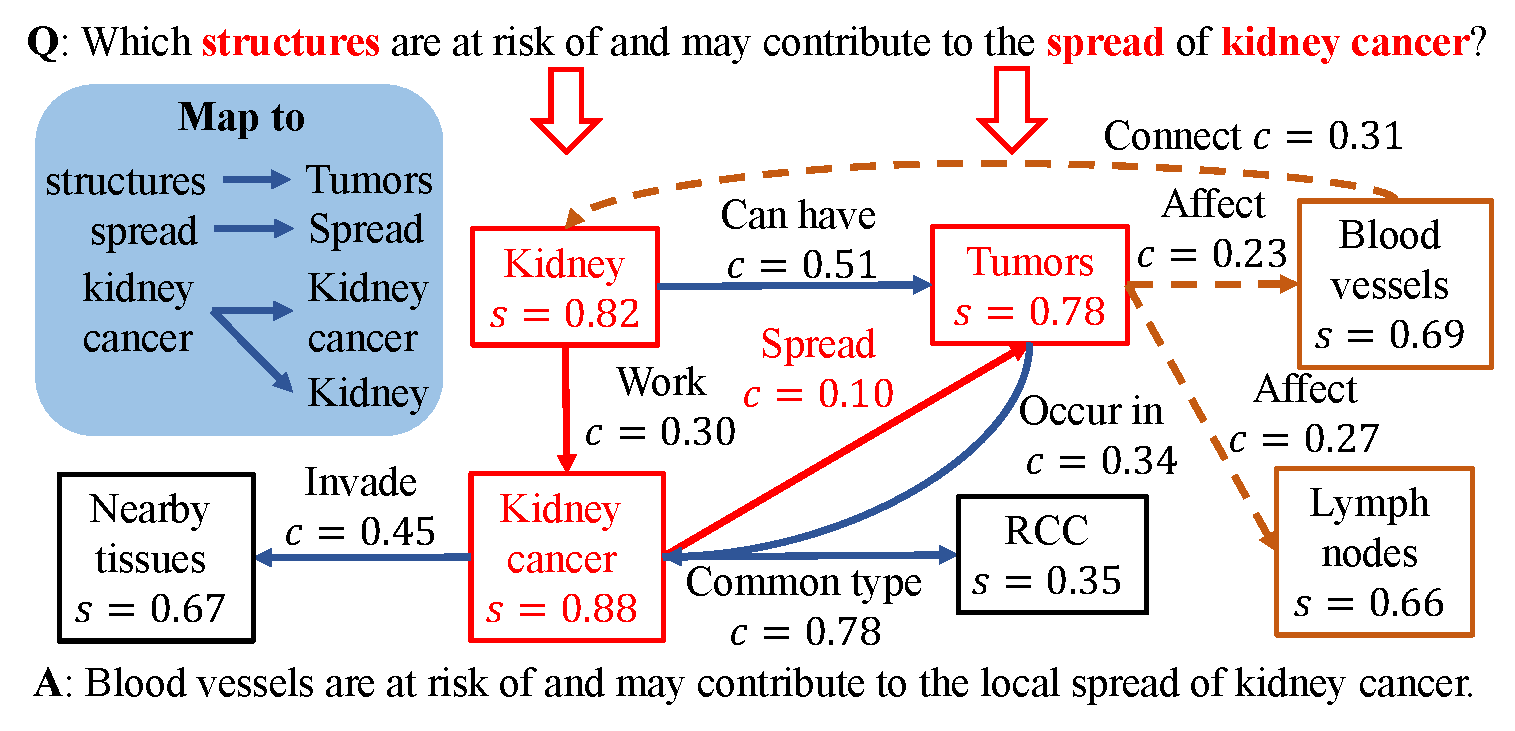
\includegraphics[width=0.88\textwidth]{figures/agrag/GERAG_example.pdf}
\caption{The original AGRAG evidence-expansion example. Red triples are query-mapped facts; orange triples show additional neighboring evidence in the illustrated MCMI structure. Reproduced from Figure 2 of the source paper~\cite{agrag-paper}.}
\label{fig:agrag:example}
\end{figure}

The theoretical claims have distinct scopes. The main paper reports NP-hardness for the stated subgraph optimization problem and a 2-approximation result for the initial terminal-connecting stage. The expansion procedure adds further evidence after that stage. Its empirical contribution is evaluated by replacing the expanded subgraph with the initial Steiner-tree representation. The chapter uses this ablation to assess the role of expansion in the evaluated tasks.
% Editorial record: the supplementary monotonic-decrease argument conflicts with the sum objective; see planning/verification-agrag.md. Do not promote it to a new theorem.

The graph returned by retrieval is serialized as $g=\operatorname{StrConcat}(\mathcal{V}_{\mathrm{MCMI}},\mathcal{E}_{\mathrm{MCMI}})$. This representation contains the selected entities and relations. It makes the selected relationships available within the model's input sequence. The graph records relationships in the indexed evidence; the generated answer remains the language model's response conditioned on that evidence.

\section{Hybrid Retrieval and Generation}
\label{sec:agrag:hybrid}
A graph index captures extracted relationships, whereas many details remain in the original text. AGRAG therefore also retrieves chunks through a hybrid score,
\begin{equation}
\operatorname{HS}(q,t)=\frac{\operatorname{MS}(\mathbf{q},\mathbf{t})+
\operatorname{BM25}(q,t)}{2},
\label{eq:agrag:hybrid}
\end{equation}
where $\mathbf{t}$ is the dense representation of chunk $t$. The top $k_r$ chunks according to this score form $\mathcal{T}_{\mathrm{HR}}$. The source reports $k_r=5$ in the main setting.

The two components of the score respond to different kinds of correspondence. Dense similarity compares distributed representations of a query and passage. BM25 responds to lexical overlap and term weighting. AGRAG averages the two scores as specified in the paper, then combines the selected chunks with the graph serialization. The hybrid channel is therefore an additional source of passage context rather than a separate graph expansion rule.

The final answer is generated through
\begin{equation}
A_q=\operatorname{LLM}(q,g,\mathcal{T}_{\mathrm{HR}},p_{\mathrm{gen}}).
\label{eq:agrag:generation}
\end{equation}
This input has a query, an explicit selected relational structure, and supporting passage content. The graph identifies connected facts. The passage channel supplies contextual language that graph extraction may omit. The ablations test both a graph-only condition and a hybrid-only condition, allowing the evaluation to distinguish their contributions.

For classification, the retrieval interface is adapted to return candidate labels associated with passages. One training passage per label supplies the indexed corpus. The generator selects a label from the retrieved candidate set. This setting shares the evidence-selection principle with the QA tasks, but its output and accuracy calculation are different. It is also distinct from GORAG's round-based online indexing protocol, which is examined in Chapter~\ref{ch:gorag}.

\section{Computational Properties}
\label{sec:agrag:complexity}
AGRAG's work is distributed across corpus indexing and query processing. Statistical extraction and passage-link construction operate over the corpus. Query processing includes triple mapping, filtering, graph propagation, subgraph selection, hybrid retrieval, and generation. Language-model calls contribute to relation extraction during indexing and to filtering and answer generation online.

The source's graph-operation analysis assigns $O(|\mathcal{V}||\mathcal{T}_c|)$ time to entity extraction and passage association. Graph propagation is expressed in terms of node and edge counts, and semantic edge weighting visits the indexed edges. The Mehlhorn-based initial tree stage is reported with $O(|\mathcal{E}|+|\mathcal{V}|\log|\mathcal{V}|)$ complexity. Expansion additionally depends on the selected subgraph and its neighborhood. These expressions characterize graph operations; the measured end-to-end results include model inference under the experimental configuration.

The distinction between indexing and querying is useful in deployment. An index is prepared once for a fixed corpus, while query filtering and generation recur for each query. An application with many queries can amortize index preparation, but its response latency still depends on online graph processing and the amount of generated text. Token counts and separate indexing/querying times are therefore retained in the evaluation.

The evidence graph also requires storage for entity strings, relations, and passage associations. The source gives storage in terms of graph nodes, edges, and text chunks. The thesis retains those objects explicitly rather than treating a graph as a cost-free representation. Practical storage depends on how embeddings, text, and adjacency structures are represented, while the experimental efficiency table reports time and token use rather than a measured memory comparison.

\section{Experimental Evaluation}
\label{sec:agrag:experiments}
\subsection{Tasks, corpora, and model settings}
The main experiment uses Novel and Medical from GraphRAG-bench, together with WOS and IFS-Rel for classification. Novel contains 5,140 chunks, 63,887 graph entities, and 163,169 graph relations. Medical contains 1,030 chunks, 12,426 entities, and 52,054 relations. The reported classification indexes contain 24 chunks for WOS and 11 for IFS-Rel, with 9,396 and 2,560 evaluated texts and 133 and 64 labels, respectively. These statistics are retained as reported in the source dataset table.

The Novel evaluation contains 67 creative-generation queries, 362 contextual-summarization queries, 610 complex-reasoning queries, and 971 fact-retrieval queries. The corresponding Medical counts are 166, 289, 509, and 1,098. Their differing sizes and answer requirements are relevant to interpretation. The chapter compares methods within each reported task and corpus rather than treating these query collections as interchangeable observations.

The main backbone is Qwen2.5-14B-Instruct, deployed through vLLM. The machine has an Intel Xeon Gold 5220R CPU and one NVIDIA A100 GPU with 80 GB memory. Contriever supplies dense representations for AGRAG and HippoRAG2; the other baselines use bge-large-en-v1.5 according to the reported configuration. Qwen3-Reranker-0.6B performs raw-triplet filtering. The retrieval top-$k$ setting is 5; AGRAG's raw mapped triple count and hybrid chunk count are also 5.

GraphRAG uses local search. LightRAG uses hybrid search for the QA tasks, with its classification-specific configuration retained where applicable. The comparison includes NaiveRAG, LongLLMLingua, RAPTOR, SiReRAG, G-Retriever, MIXRAG, GraphRAG, LightRAG, HippoRAG2, and Fast-GraphRAG. These methods represent passage retrieval, compression, hierarchical organization, connected subgraph selection, neighborhood retrieval, and graph propagation. The source experiments compare their complete configurations under the stated model settings.

\subsection{Metric interpretation}
Classification accuracy is the proportion of predicted labels matching gold labels. Classification recall is macro recall. For the other tasks, the reported accuracy is a model-assessed score with values 0, 0.5, or 1 for inaccurate, partially accurate, or accurate answers. These quantities appear under the same ACC heading in the paper but evaluate different outputs.

Complex reasoning and fact retrieval additionally report the source's ROUGE-L measure. Contextual summarization and creative generation report coverage, the fraction of required reference evidence represented in the answer. Creative generation also reports faithfulness, the fraction of answer claims supported by retrieved context. The source uses the RAGAS framework and its task-specific evaluation protocol. Coverage concerns inclusion of required information, whereas faithfulness concerns support for generated claims.

These distinctions explain why multiple metrics are retained. A response can cover many reference items while adding unsupported claims, or remain grounded while omitting part of the required answer. A classification system can retrieve useful candidates but still select the wrong label. The evaluation therefore reports the actual task metrics instead of deriving a common aggregate score across QA and classification.

\begin{table}[tbp]
\centering
\small
\setlength{\tabcolsep}{3pt}
\caption{Creative generation results from the main AGRAG experiment with Qwen2.5-14B-Instruct. Values and emphasis reproduce the corresponding columns of the source paper\cite{agrag-paper}, Table III.}
\label{tab:agrag:main-creative}
\resizebox{\textwidth}{!}{%
\begin{tabular}{lrrrrrr}
\toprule
Method & Novel FS & Novel ACC & Novel COV & Medical FS & Medical ACC & Medical COV\\
\midrule
NaiveRAG & 0.205 & 0.307 & \uline{0.384} & 0.176 & \uline{0.577} & \uline{0.554}\\
L.LLMLingua & 0.213 & 0.316 & 0.377 & 0.225 & 0.575 & 0.496\\
RAPTOR & 0.365 & \uline{0.333} & 0.373 & 0.314 & 0.526 & 0.553\\
SiReRAG & 0.324 & 0.328 & 0.365 & 0.295 & 0.544 & 0.456\\
G-retriever & 0.294 & 0.167 & 0.200 & 0.169 & 0.371 & 0.468\\
MIXRAG & 0.200 & 0.286 & 0.337 & 0.255 & 0.351 & 0.306\\
GraphRAG & 0.427 & 0.310 & 0.339 & 0.345 & 0.475 & 0.325\\
LightRAG & 0.201 & 0.314 & 0.329 & 0.189 & 0.567 & 0.549\\
HippoRAG2 & \uline{0.496} & 0.295 & 0.325 & \uline{0.347} & 0.563 & 0.451\\
F.GraphRAG & 0.286 & 0.287 & 0.376 & 0.217 & 0.500 & 0.396\\
\textbf{AGRAG} & \textbf{0.513} & \textbf{0.339} & \textbf{0.386} & \textbf{0.356} & \textbf{0.598} & \textbf{0.589}\\
\bottomrule
\end{tabular}}
\end{table}

\begin{table}[tbp]
\centering
\small
\setlength{\tabcolsep}{3pt}
\caption{Contextual summarization results from the main AGRAG experiment with Qwen2.5-14B-Instruct. Values and emphasis reproduce the corresponding columns of the source paper\cite{agrag-paper}, Table III.}
\label{tab:agrag:main-summary}
\resizebox{\textwidth}{!}{%
\begin{tabular}{lrrrr}
\toprule
Method & Novel COV & Novel ACC & Medical COV & Medical ACC\\
\midrule
NaiveRAG & 0.745 & 0.621 & \uline{0.677} & 0.576\\
L.LLMLingua & 0.687 & 0.627 & 0.657 & 0.583\\
RAPTOR & \uline{0.760} & 0.626 & 0.633 & 0.583\\
SiReRAG & 0.754 & 0.617 & 0.592 & 0.560\\
G-retriever & 0.594 & 0.404 & 0.302 & 0.395\\
MIXRAG & 0.695 & 0.538 & 0.409 & 0.464\\
GraphRAG & 0.758 & 0.620 & 0.625 & 0.506\\
LightRAG & 0.753 & \uline{0.628} & 0.625 & 0.585\\
HippoRAG2 & 0.735 & 0.586 & 0.496 & 0.560\\
F.GraphRAG & 0.706 & 0.528 & 0.507 & \uline{0.587}\\
\textbf{AGRAG} & \textbf{0.778} & \textbf{0.643} & \textbf{0.690} & \textbf{0.604}\\
\bottomrule
\end{tabular}}
\end{table}

\begin{table}[tbp]
\centering
\small
\setlength{\tabcolsep}{3pt}
\caption{Complex reasoning results from the main AGRAG experiment with Qwen2.5-14B-Instruct. Values and emphasis reproduce the corresponding columns of the source paper\cite{agrag-paper}, Table III.}
\label{tab:agrag:main-complex}
\resizebox{\textwidth}{!}{%
\begin{tabular}{lrrrr}
\toprule
Method & Novel ROG & Novel ACC & Medical ROG & Medical ACC\\
\midrule
NaiveRAG & 0.120 & 0.447 & 0.117 & 0.635\\
L.LLMLingua & 0.092 & 0.434 & 0.080 & 0.633\\
RAPTOR & 0.290 & \uline{0.460} & 0.185 & \uline{0.649}\\
SiReRAG & 0.307 & 0.459 & 0.269 & 0.646\\
G-retriever & 0.146 & 0.441 & 0.102 & 0.396\\
MIXRAG & 0.109 & 0.386 & 0.156 & 0.434\\
GraphRAG & 0.246 & 0.449 & 0.250 & 0.606\\
LightRAG & 0.223 & 0.448 & 0.255 & 0.637\\
HippoRAG2 & \uline{0.314} & 0.453 & \uline{0.332} & 0.622\\
F.GraphRAG & 0.237 & 0.371 & 0.262 & 0.643\\
\textbf{AGRAG} & \textbf{0.319} & \textbf{0.467} & \textbf{0.343} & \textbf{0.665}\\
\bottomrule
\end{tabular}}
\end{table}

\begin{table}[tbp]
\centering
\small
\setlength{\tabcolsep}{3pt}
\caption{Fact retrieval results from the main AGRAG experiment with Qwen2.5-14B-Instruct. Values and emphasis reproduce the corresponding columns of the source paper\cite{agrag-paper}, Table III.}
\label{tab:agrag:main-fact}
\resizebox{\textwidth}{!}{%
\begin{tabular}{lrrrr}
\toprule
Method & Novel ROG & Novel ACC & Medical ROG & Medical ACC\\
\midrule
NaiveRAG & 0.117 & 0.431 & 0.182 & 0.604\\
L.LLMLingua & 0.115 & 0.420 & 0.105 & 0.591\\
RAPTOR & 0.133 & 0.465 & 0.132 & 0.609\\
SiReRAG & 0.311 & 0.451 & 0.349 & 0.558\\
G-retriever & 0.199 & 0.209 & 0.148 & 0.326\\
MIXRAG & 0.102 & 0.366 & 0.160 & 0.463\\
GraphRAG & 0.240 & 0.445 & 0.217 & 0.521\\
LightRAG & 0.253 & 0.460 & 0.283 & 0.607\\
HippoRAG2 & 0.310 & \uline{0.470} & 0.343 & 0.598\\
F.GraphRAG & \uline{0.318} & 0.439 & \uline{0.352} & \uline{0.610}\\
\textbf{AGRAG} & \textbf{0.324} & \textbf{0.490} & \textbf{0.357} & \textbf{0.628}\\
\bottomrule
\end{tabular}}
\end{table}

\begin{table}[tbp]
\centering
\small
\setlength{\tabcolsep}{3pt}
\caption{Text classification results from the main AGRAG experiment with Qwen2.5-14B-Instruct. Values and emphasis reproduce the corresponding columns of the source paper\cite{agrag-paper}, Table III.}
\label{tab:agrag:main-class}
\resizebox{\textwidth}{!}{%
\begin{tabular}{lrrrr}
\toprule
Method & WOS ACC & WOS REC & IFS-REL ACC & IFS-REL REC\\
\midrule
NaiveRAG & 0.237 & 0.257 & 0.351 & 0.197\\
L.LLMLingua & 0.274 & 0.231 & 0.378 & 0.220\\
RAPTOR & 0.409 & 0.290 & 0.293 & 0.212\\
SiReRAG & \uline{0.430} & \uline{0.294} & 0.325 & 0.220\\
G-retriever & 0.188 & 0.129 & 0.311 & 0.185\\
MIXRAG & 0.244 & 0.235 & 0.362 & 0.203\\
GraphRAG & 0.253 & 0.201 & 0.279 & 0.202\\
LightRAG & 0.273 & 0.224 & 0.265 & 0.220\\
HippoRAG2 & 0.424 & 0.270 & \uline{0.389} & \uline{0.246}\\
F.GraphRAG & 0.283 & 0.245 & 0.307 & 0.221\\
\textbf{AGRAG} & \textbf{0.438} & \textbf{0.307} & \textbf{0.403} & \textbf{0.251}\\
\bottomrule
\end{tabular}}
\end{table}


\subsection{Answer quality across tasks}
The main results are split by task in Tables~\ref{tab:agrag:main-creative}--\ref{tab:agrag:main-class}. On Novel creative generation, AGRAG reports faithfulness 0.513, accuracy 0.339, and coverage 0.386. HippoRAG2 reports faithfulness 0.496, while RAPTOR reports accuracy 0.333 and NaiveRAG coverage 0.384. The close coverage values and the different best comparison methods show why one baseline cannot summarize every metric.

On Medical creative generation, AGRAG reports faithfulness 0.356, accuracy 0.598, and coverage 0.589. NaiveRAG has accuracy 0.577 and coverage 0.554. HippoRAG2 has faithfulness 0.347. The task combines contextual grounding with a more flexible response format, and the three measures capture different aspects of that response. The reported improvements concern this protocol and corpus.

For contextual summarization, AGRAG obtains coverage and accuracy of 0.778 and 0.643 on Novel, and 0.690 and 0.604 on Medical. The task requires collecting information distributed across the evidence. The result is consistent with the design of supplying connected graph facts together with passage context. The ablations provide the more direct component comparison by removing either the graph structure or the hybrid channel.

For complex reasoning, the reported ROUGE-L and accuracy values are 0.319 and 0.467 on Novel and 0.343 and 0.665 on Medical. For fact retrieval they are 0.324 and 0.490 on Novel and 0.357 and 0.628 on Medical. The differences between tasks are expected from their distinct questions and answer formats. These scores should be compared to the corresponding baseline column rather than used to rank the intrinsic difficulty of the corpora.

Classification accuracy and recall are 0.438 and 0.307 on WOS and 0.403 and 0.251 on IFS-Rel. SiReRAG reports WOS accuracy 0.430 and recall 0.294, while HippoRAG2 reports IFS-Rel accuracy 0.389 and recall 0.246. AGRAG's classifier receives graph-derived candidate labels under the source protocol. The results evaluate the combined retrieval and label-selection pipeline, so improvements cannot be assigned solely to the final language-model decision.

\subsection{Indexing and querying costs}
\begin{table}[t]
	\centering
	\renewcommand{\arraystretch}{1.2}
	\caption{Model efficiency on 4 datasets for 5 tasks, all experiments were carried out with Qwen2.5-14B-Instruct LLM backbone. 
		
	}
	\label{tab:agrag:efficiency}
	
	\setlength\tabcolsep{1pt}
 
		\resizebox{\textwidth}{!}{%
\begin{tabular}{l|l|cccc|cccc} 
			\hline\hline
			\multirow{2}{*}{\textbf{Category}}                                             & \multirow{2}{*}{\textbf{Models}} & \multicolumn{4}{c|}{\textbf{Time Cost (Indexing / Querying mins) }}           & \multicolumn{4}{c}{\textbf{Token Cost (Input / Output per query) }}                                             \\ 
			\cline{3-10}
			&                                  & \textbf{Novel}    & \textbf{Medical}  & \textbf{WOS}      & \textbf{IFS-REL}  & \textbf{Novel}               & \textbf{Medical}             & \textbf{WOS}               & \textbf{IFS-REL}     \\ 
			\hline\hline
			\multirow{2}{*}{\begin{tabular}[c]{@{}l@{}}Traditional\\RAG\end{tabular}}
}      & NaiveRAG                         & \textbf{13} / 371 & \textbf{7} / 245  & \textbf{2} / 292  & \textbf{2} / 225  & 9,437 / 1,708                & 7,473 / 379                  & 7,292 / 29                  & 4,521 / \underline{16}   \\
			& L.LLMLingua                      & 51 / 360          & 37 / 305          & \underline{4} / 358   & \underline{3} / 315   & 8,466 / 1,750                & 5,686 / 390                  & 5,861 / \underline{31}         & 2,757 / \textbf{14}  \\ 
			\hline
			\multirow{2}{*}{\begin{tabular}[c]{@{}l@{}}Tree\\-based RAG\end{tabular}}      & RAPTOR                           & 464 / 250         & 117 / 319         & 30 / 162          & 24 / \textbf{121} & 7,243 / 777                  & \underline{4,817} / 695          & 6,007 / 41                 & 3,807 / 33           \\
			& SiReRAG                          & 85 / 233          & 40 / 207          & 26 / 139          & 18 / 117          & 7,759 / 800                  & 4,918 / 701                  & 6,012 / 47                 & 3,821 / 36           \\ 
			\hline
			\multirow{4}{*}{\begin{tabular}[c]{@{}l@{}}Community\\-based RAG\end{tabular}} & G-Retriever                      & 19 / \textbf{119} & 12 / 145          & 8 / \underline{158}   & \underline{3} / 164   & \underline{6,344} / \textbf{116} & 6,290 / \textbf{157}         & 6,762 / \textbf{12}        & 4,002 / 21           \\
			& MIXRAG                           & \underline{17} / 388  & \underline{11} / 453  & 5 /  257          & \textbf{2} / 193  & \textbf{6,083} / \underline{237} & \textbf{4,238 }/ \underline{230} & \underline{4,193 }/ \underline{31} & 3,597 / 29           \\
			& GraphRAG                         & 347 / 205         & 194 / 158         & 85 / 240          & 64 / 217          & 12,686 / 2,109               & 8,385 / 1,017                & 11,809 / 351               & 9,009 / 287          \\
			& LightRAG                         & 166 / 221         & 116 / 164         & 42 / 211          & 31 / 197          & 13,145 / 1,233               & 9,535 / 426                  & 11,510 / 227               & 7,667 / 199          \\ 
			\hline
			\multirow{3}{*}{\begin{tabular}[c]{@{}l@{}}Walking\\-based RAG~\end{tabular}}  & HippoRAG2                        & 95 / \underline{134}  & 46 / \textbf{130} & 19 / 140          & 15 / 127          & 8,138 / 1,073                & 6,264 / 595                  & 5,066 / 93                 & 2,440 / 102          \\
			& F.GraphRAG                       & 106 / 198         & 48 / 173          & 29 / 186          & 27 / 164          & 7,490 / 1,252                & 6,475 / 384                  & 4,957 / 35                 & \underline{2,217} / 20   \\
			& \textbf{AGRAG}                   & 65 / 142          & 16 / \underline{138}  & 16 / \textbf{132} & 14 / \underline{124}  & 6,487 / 1,140                & 5,145 / 413                  & \textbf{3,970} / 101       & \textbf{1,890} / 93  \\
			\hline\hline
		\end{tabular}
		
	
\end{table}

Table~\ref{tab:agrag:efficiency} separates indexing time, querying time, input tokens, and output tokens. For Novel, AGRAG reports 65 minutes for indexing and 142 minutes for querying, compared with HippoRAG2's 95 and 134 minutes. For Medical the corresponding values are 16 and 138 minutes for AGRAG and 46 and 130 minutes for HippoRAG2. This comparison shows lower index preparation time alongside a higher reported query total for AGRAG.

The table also contains methods with lower costs in particular columns. NaiveRAG has lower indexing times, while G-Retriever has a shorter Novel querying total. AGRAG's efficiency therefore needs to be read together with the task results and the individual cost components. The evidence supports a quality--cost comparison under the shared configuration rather than a claim that one system minimizes every resource measure.

On WOS and IFS-Rel, AGRAG reports querying times of 132 and 124 minutes and input token counts of 3,970 and 1,890 per query. The corresponding HippoRAG2 values are 140 and 127 minutes and 5,066 and 2,440 tokens. Output lengths differ between methods. Preserving both input and output counts helps distinguish the amount of supplied evidence from the cost of producing an answer.

\subsection{Component ablations}
\begin{table}
	\centering
	\caption{The ablation experiment result on the two datasets and 4 tasks. All experiments were carried out with Qwen2.5-14B-Instruct LLM, where Time (I / Q) denotes the Index and Query time, Token (I / O) denotes the LLM Input and Output token count.}
	\label{tab:agrag:ablation}
	\setlength\tabcolsep{1.5pt}
	\resizebox{\linewidth}{!}{
		\begin{tabular}{l|ccc|ccc|cc|cc|cc|cc|cc|cc|cc|cc} 
			\hline\hline
			\multirow{3}{*}{\textbf{Model }} & \multicolumn{6}{c|}{\textbf{Creative Gen. }}                                                        & \multicolumn{4}{c|}{\textbf{Contextual Sum. }}                              & \multicolumn{4}{c|}{\textbf{Complex Rea. }}                                 & \multicolumn{4}{c|}{\textbf{Fact Retrieval }}                               & \multicolumn{4}{c}{\textbf{Model Efficiency }}                                                                             \\ 
			\cline{2-23}
			& \multicolumn{3}{c|}{\textbf{Novel }}             & \multicolumn{3}{c|}{\textbf{Medical }}           & \multicolumn{2}{c|}{\textbf{Novel}} & \multicolumn{2}{c|}{\textbf{Medical}} & \multicolumn{2}{c|}{\textbf{Novel}} & \multicolumn{2}{c|}{\textbf{Medical}} & \multicolumn{2}{c|}{\textbf{Novel}} & \multicolumn{2}{c|}{\textbf{Medical}} & \multicolumn{2}{c|}{\textbf{Novel }}                         & \multicolumn{2}{c}{\textbf{Medical }}                       \\ 
			\cline{2-23}
			& \textbf{FS.}   & \textbf{ACC.}  & \textbf{COV.}  & \textbf{FS.}   & \textbf{ACC.}  & \textbf{COV.}  & \textbf{COV. } & \textbf{ACC.}      & \textbf{COV.}  & \textbf{ACC.}        & \textbf{ROG.}  & \textbf{ACC.}      & \textbf{ROG.}  & \textbf{ACC.}        & \textbf{ROG.}  & \textbf{ACC.}      & \textbf{ROG.}  & \textbf{ACC.}        & \textbf{Time (I / Q)}         & \textbf{Token (I / G)}       & \textbf{Time (I / Q)}        & \textbf{Token (I / G)}       \\ 
			\hline\hline
			AGRAG w. HR Only                 & 0.491          & \underline{0.322}  & 0.378          & 0.303          & 0.526          & 0.549          & 0.739          & 0.522              & 0.535          & 0.583                & 0.303          & 0.453              & 0.334          & \underline{0.636}        & \underline{0.323}  & \underline{0.487}      & 0.355          & 0.619                & \textbf{11.7} / \underline{137.9} & \textbf{5,117} / \underline{193} & 11.4 / \underline{117.9}         & \underline{5,215} / \underline{199}  \\
			AGRAG w. LLM ER                  & 0.428          & 0.302          & \underline{0.365}  & 0.352          & 0.526          & \underline{0.587}  & \underline{0.755}  & 0.552              & 0.600          & 0.566                & \underline{0.320}  & \underline{0.465}      & 0.333          & 0.624                & 0.322          & 0.480              & 0.353          & 0.613                & 83.3 /  161.2                 & 8,030 /   887                & 31.9 / 148.8                 & 5,457  / 414                 \\
			AGRAG w.o. HR                    & \textbf{0.519} & 0.306          & 0.343          & 0.342          & 0.521          & 0.570          & 0.677          & 0.534              & 0.420          & 0.578                & 0.318          & 0.434              & 0.324          & 0.598                & 0.314          & \underline{0.487}      & 0.344          & 0.615                & \underline{61.7} / 138.9          & 6,986 / 741                  & \underline{9.4 }/ \textbf{114.4} & \textbf{4,820} / 315         \\
			AGRAG w.o. MCMI                  & 0.488          & \underline{0.332}  & 0.358          & \underline{0.351}  & \underline{0.530}  & 0.575          & 0.748          & \underline{0.592}      & 0.600          & \underline{0.588}        & \textbf{0.324} & \underline{0.465}      & 0.329          & 0.633                & 0.322          & 0.470              & \textbf{0.359} & \underline{0.621}        & 63.9 / \textbf{130.4}         & \underline{6,710} / 757          & 9.5 /  125.0                 & 5,230 /    331               \\
			AGRAG w.o. Cle.                  & 0.478          & 0.311          & 0.361          & 0.336          & 0.517          & 0.569          & 0.712          & 0.597              & \underline{0.616}  & 0.577                & 0.301          & 0.450              & \underline{0.334}  & 0.628                & 0.313          & 0.478              & 0.354          & 0.620                & 65.6 / 140.1                  & 6,988 / \textbf{154}         & 9.1 / 142.9                  & 5,252 / \textbf{158}         \\
			
			\textbf{AGRAG}                   & \underline{0.513}  & \textbf{0.339} & \textbf{0.386} & \textbf{0.356} & \textbf{0.598} & \textbf{0.589} & \textbf{0.778} & \textbf{0.643}     & \textbf{0.690} & \textbf{0.604}       & 0.319          & \textbf{0.467}     & \textbf{0.343} & \textbf{0.665}       & \textbf{0.324} & \textbf{0.490}     & \underline{0.357}  & \textbf{0.628}       & 65.6 / 142.0                  & 6,988 / 639                  & \textbf{9.1} / 145.3         & 5,252 / 306                  \\
			\hline\hline
		\end{tabular}
	}
	
\end{table}

The ablation compares hybrid retrieval alone, language-model entity extraction, graph retrieval without hybrid context, an initial tree without MCMI expansion, and retrieval without the raw-triplet filtering step. These interventions act on different parts of the pipeline. They therefore give more specific evidence than the comparison between complete systems.

The hybrid-only variant has Novel creative-generation faithfulness 0.491, accuracy 0.322, and coverage 0.378. Full AGRAG reports 0.513, 0.339, and 0.386. For Novel contextual summarization, hybrid-only coverage and accuracy are 0.739 and 0.522, compared with 0.778 and 0.643 for the complete system. The graph-containing configuration provides an observed benefit under these settings, particularly for the summarization accuracy score.

Removing hybrid retrieval produces a different pattern. Novel creative-generation faithfulness is 0.519, exceeding the complete system's 0.513, while accuracy and coverage decrease to 0.306 and 0.343. Medical contextual-summarization coverage decreases from 0.690 to 0.420. The graph-only variant can produce well-grounded claims while supplying less of the required information. This is why the chapter retains both faithfulness and coverage rather than summarizing the ablation as uniform improvement.

Replacing statistical entity extraction with model-based extraction gives Novel creative-generation faithfulness 0.428 and accuracy 0.302, with indexing time 83.3 minutes in the ablation setting. The complete configuration reports 65.6 minutes in that table. This experiment changes entity extraction while retaining the rest of the method. It measures the downstream consequence of that replacement; the aggregate scores alone do not identify every intermediate graph error.

The variant without MCMI expansion uses a Steiner-tree representation. Its Novel contextual-summarization accuracy is 0.592, compared with 0.643 for full AGRAG, and its Medical creative-generation accuracy is 0.530, compared with 0.598. Some fact-retrieval metrics are close or favor the tree variant. Expansion is thus most informative in the evaluated tasks that require gathering and combining additional evidence, while the table preserves cases where the simpler representation performs similarly.

Removing raw-triplet filtering gives Novel contextual-summarization coverage 0.712 and accuracy 0.597. These are below 0.778 and 0.643 for full AGRAG. The ablation evaluates whether the initial semantic mapping alone supplies appropriate query anchors. Its results support retaining the filtering stage under the reported configuration. They do not require a separate claim that every filtered triple would otherwise cause an incorrect answer.

The ablation and main efficiency tables use separate reported measurements. For example, the Medical indexing/querying totals differ between the tables. Both sets of values are retained in their original experimental contexts. They are not averaged or substituted for one another when discussing a component intervention.

\subsection{Additional resource setting and parameter study}
\begin{table}
	\centering
	\caption{Low resource experiment effectiveness with Qwen3-4B-Instruct-2507 LLM on 2080Ti GPU, where model with -L denotes low resource setting.}
	\label{tab:agrag:low-resource}
	
	\setlength\tabcolsep{1.5pt}{
		\resizebox{\textwidth}{!}{%
\begin{tabular}{l|ccc|ccc|cc|cc|cc|cc|cc|cc} 
			\hline\hline
			\textbf{Task}    & \multicolumn{6}{c|}{\textbf{Creative Gen. }}                                                        & \multicolumn{4}{c|}{\textbf{Contextual Sum. }}                                & \multicolumn{4}{c|}{\textbf{Complex Rea. }}                                   & \multicolumn{4}{c}{\textbf{Fact Retrieval }}                                  \\ 
			\hline
			\textbf{Dataset} & \multicolumn{3}{c|}{\textbf{Novel }}             & \multicolumn{3}{c|}{\textbf{Medical }}           & \multicolumn{2}{c|}{\textbf{Novel }} & \multicolumn{2}{c|}{\textbf{Medical }} & \multicolumn{2}{c|}{\textbf{Novel }} & \multicolumn{2}{c|}{\textbf{Medical }} & \multicolumn{2}{c|}{\textbf{Novel }} & \multicolumn{2}{c}{\textbf{Medical }}  \\ 
			\hline
			\textbf{Metric}  & \textbf{FS.}   & \textbf{ACC.}  & \textbf{COV.}  & \textbf{FS.}   & \textbf{ACC.}  & \textbf{COV.}  & \textbf{COV.}  & \textbf{ACC.}       & \textbf{COV.}  & \textbf{ACC.}         & \textbf{ROG.}  & \textbf{ACC.}       & \textbf{ROG.}  & \textbf{ACC.}         & \textbf{ROG.}  & \textbf{ACC.}       & \textbf{ROG.}  & \textbf{ACC.}         \\ 
			\hline\hline
			SiReRAG-L        & 0.324          & 0.412          & 0.299          & 0.421          & \underline{0.758}  & \underline{0.475}  & 0.647          & \underline{0.673}       & \underline{0.536}  & \underline{0.738}         & 0.260          & 0.426               & \underline{0.308}  & \underline{0.698}         & 0.271          & 0.416               & \underline{0.343}  & \underline{0.661}         \\
			HippoRAG2-L      & \underline{0.433}  & \underline{0.481}  & \underline{0.335}  & \underline{0.425}  & 0.755          & 0.433          & \underline{0.696}  & 0.657               & 0.522          & 0.731                 & \underline{0.280}  & \underline{0.507}       & 0.298          & 0.681                 & \underline{0.288}  & \underline{0.513}       & 0.338          & 0.654                 \\
			\textbf{AGRAG-L} & \textbf{0.441} & \textbf{0.519} & \textbf{0.354} & \textbf{0.436} & \textbf{0.777} & \textbf{0.490} & \textbf{0.745} & \textbf{0.706}      & \textbf{0.545} & \textbf{0.751}        & \textbf{0.293} & \textbf{0.552}      & \textbf{0.312} & \textbf{0.739}        & \textbf{0.297} & \textbf{0.560}      & \textbf{0.351} & \textbf{0.701}        \\ 
			\hline\hline
			
			
			
		\end{tabular}}

	}
	
\end{table}

\begin{table}
	\centering
	\caption{Low resource experiment efficiency with Qwen3-4B-Instruct-2507 LLM on 2080Ti GPU, where -L denotes low resource setting.}
	\label{tab:agrag:low-resource-efficiency}
	\setlength\tabcolsep{1.5pt}{
		\resizebox{\textwidth}{!}{%
\begin{tabular}{l|cc|cc|cc|cc} 
			\hline\hline
			\multirow{2}{*}{\textbf{Dataset}} & \multicolumn{4}{c|}{\textbf{Novel}}                                                    & \multicolumn{4}{c}{\textbf{Medical }}                                                                  \\ 
			\cline{2-9}
			& \multicolumn{2}{c|}{\textbf{Time (mins) }} & \multicolumn{2}{c|}{\textbf{AVG.~Token }} & \multicolumn{2}{c|}{\textbf{\textbf{Time (mins)}}} & \multicolumn{2}{c}{\textbf{\textbf{AVG. Token}}}  \\ 
			\hline
			\textbf{Metric}                   & \textbf{Index} & \textbf{Query}            & \textbf{In}    & \textbf{Out}             & \textbf{\textbf{Index}} & \textbf{\textbf{Query}}  & \textbf{\textbf{In}} & \textbf{\textbf{Out}}      \\ 
			\hline\hline
			SiReRAG-L                         & \underline{52.0}   & 183.5                     & \underline{7,898}  & \textbf{1,003}           & 18.1                    & 182.3                    & \textbf{5,113}       & 827                        \\
			HippoRAG2-L                       & 55.7           & \textbf{131.2}            & 7,964          & 1,354                    & \underline{21.8}            & \textbf{162.4}           & 5,577                & \underline{584}                \\
			\textbf{AGRAG-L}                  & \textbf{44.7}  & \underline{132.1}             & \textbf{6,625} & \underline{1,172}            & \textbf{14.4}           & \underline{167.3}            & \underline{5,282}        & \textbf{534}               \\ 
			\hline\hline
			
			
			
		\end{tabular}}

	}
\end{table}

The low-resource experiment uses Qwen3-4B-Instruct-2507 on two NVIDIA 2080 Ti GPUs. This changes both model and hardware relative to the main experiment. The comparison therefore concerns the methods within that resource setting. It supplies evidence about operating with a smaller backbone and different accelerators rather than a controlled estimate of the effect of model size alone.

In that setting, AGRAG-L reports Novel creative-generation accuracy 0.519 and contextual-summarization accuracy 0.706. Its Novel index/query totals are 44.7 and 132.1 minutes. Medical totals are 14.4 and 167.3 minutes. HippoRAG2-L has shorter query totals in both corpora, while AGRAG-L has shorter indexing totals. The complete low-resource tables retain the quality and token measures needed to assess those tradeoffs.

The parameter study varies the maximum n-gram length over $\{1,3,5,7\}$ and the extraction threshold over $\{0.1,0.3,0.5,0.7\}$. The original heatmaps are reproduced in Figure~\ref{fig:agrag:sensitivity}. They show accuracy across the tested combinations for Novel and Medical. The main experiment uses $b=3$ and $\tau=0.5$. The curves and heatmaps are not converted into additional inferred numerical results.

\begin{figure}[p]
\centering
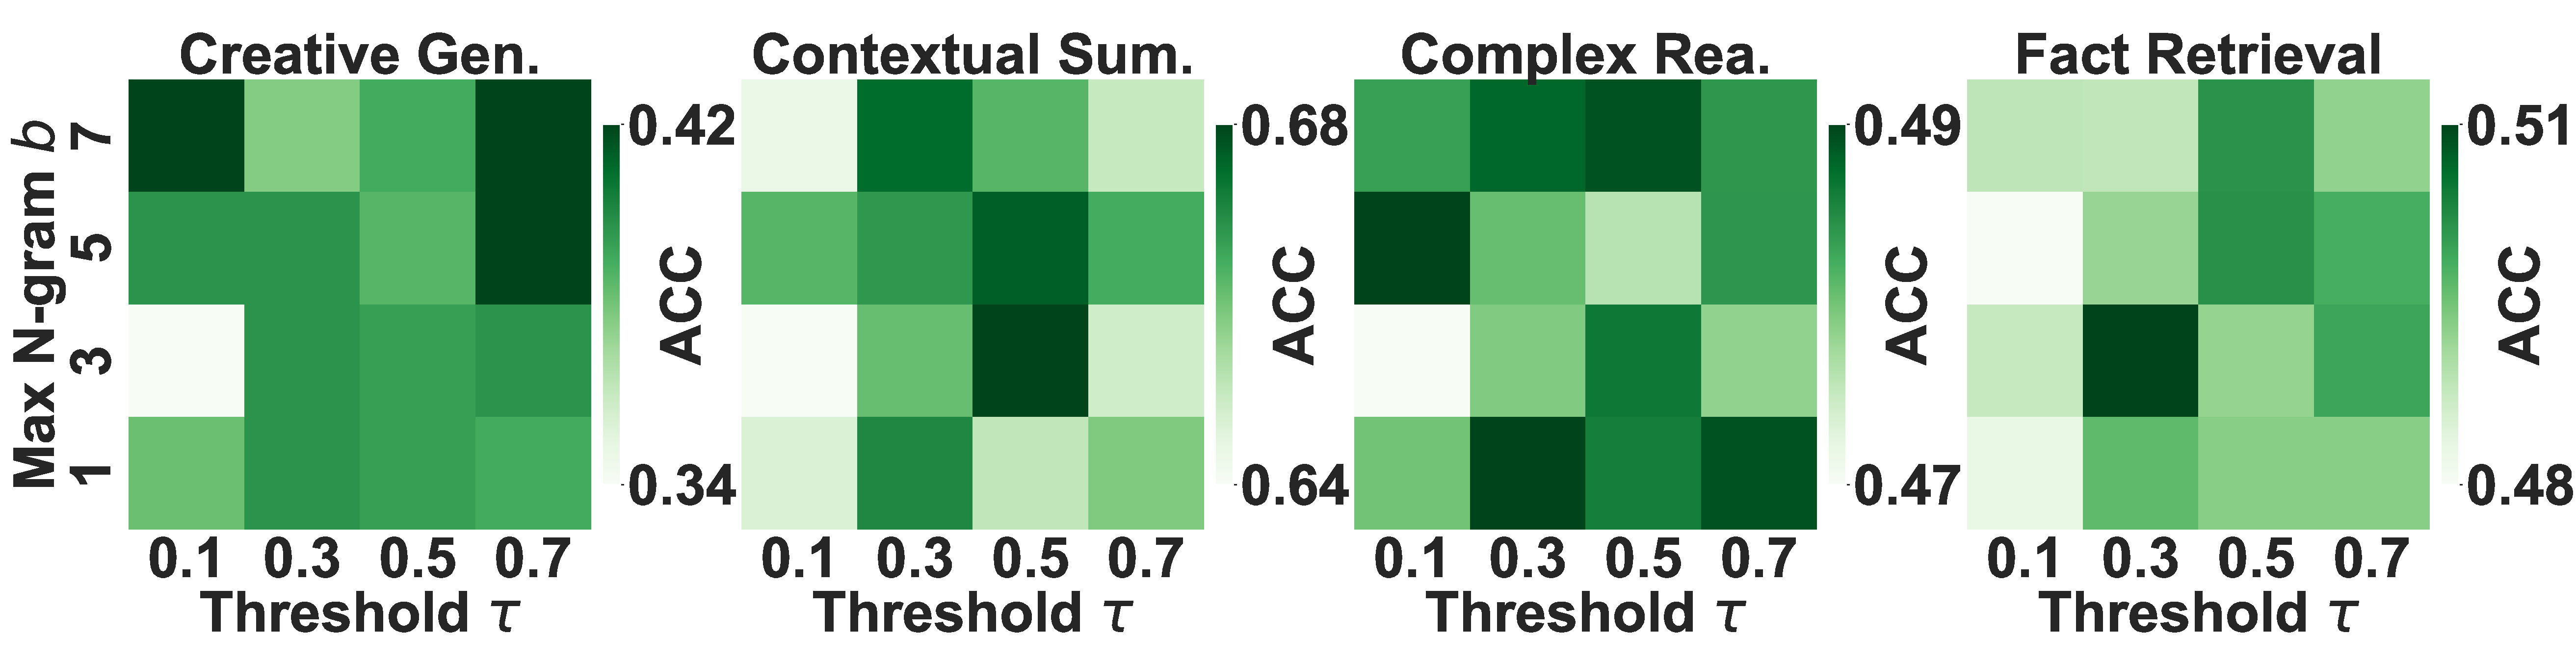
\includegraphics[width=0.95\textwidth]{figures/agrag/heatmap_novel.pdf}\\[1em]
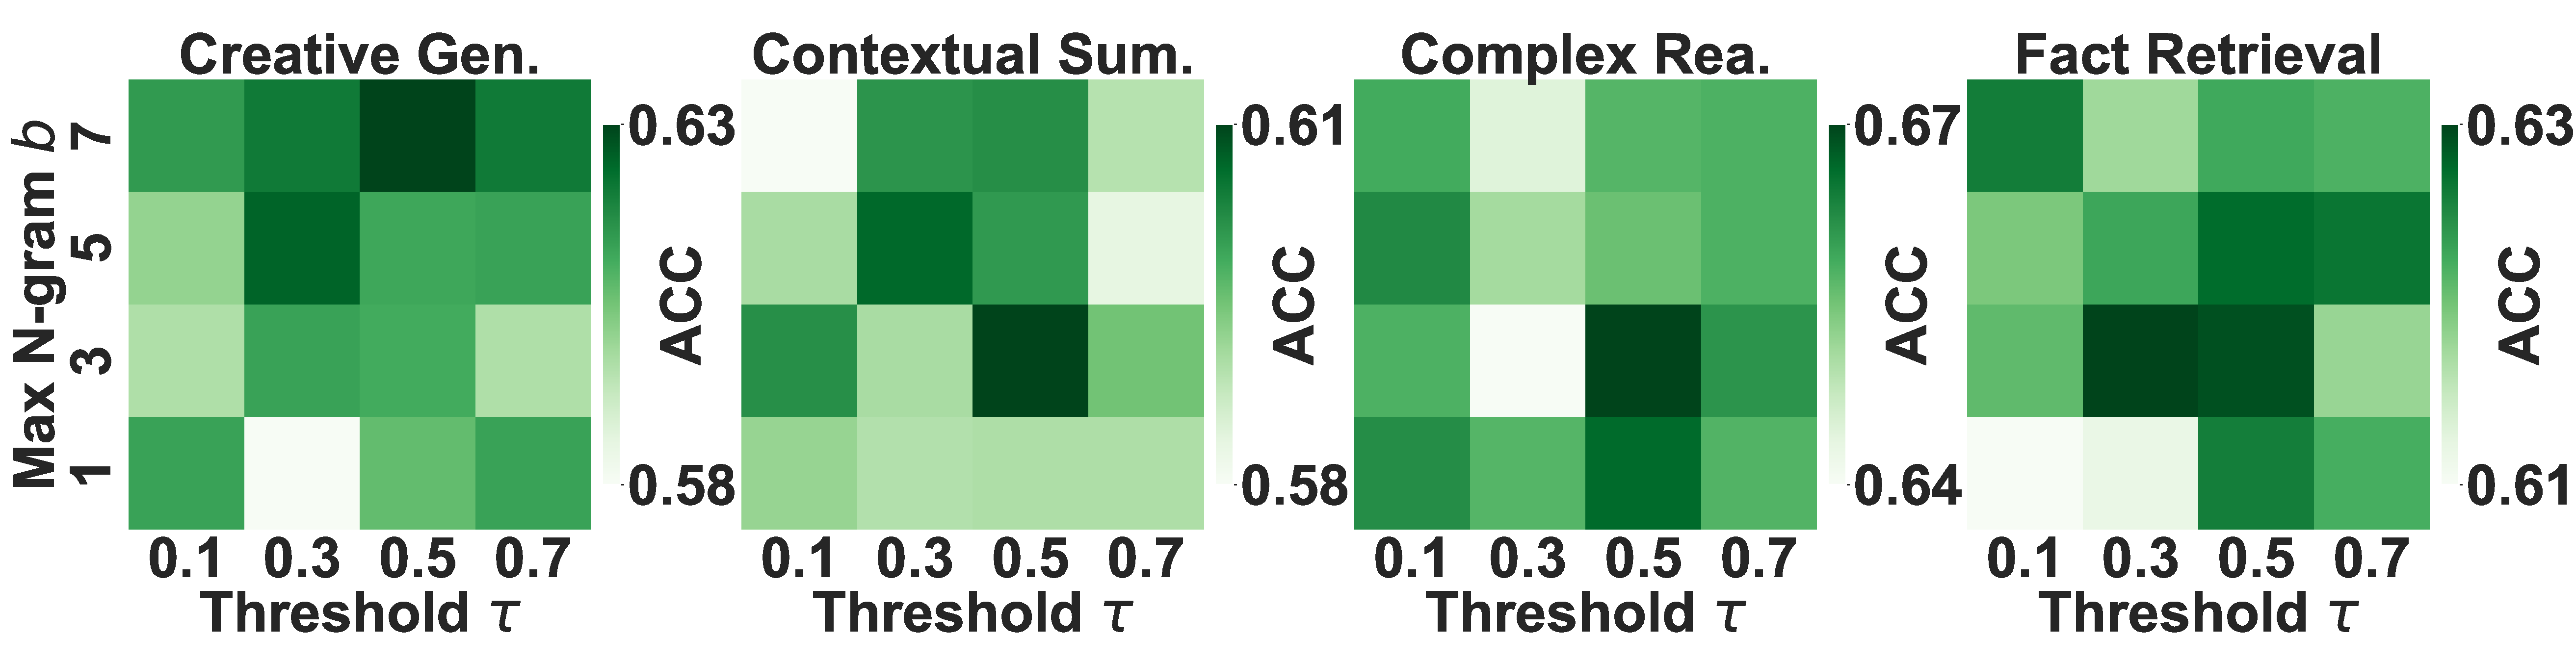
\includegraphics[width=0.95\textwidth]{figures/agrag/heatmap_medical.pdf}
\caption{AGRAG parameter sensitivity on Novel (top) and Medical (bottom). The original panels vary the extraction threshold and maximum n-gram length and display task accuracy. Reproduced from Figure 3 of the source paper~\cite{agrag-paper}.}
\label{fig:agrag:sensitivity}
\end{figure}

\section{Discussion and Chapter Summary}
\label{sec:agrag:discussion}
AGRAG places structure at two points in the evidence pipeline. Graph construction determines which entities, relations, and passage links are available. Query-time selection determines how those items are connected in the context supplied to the generator. The hybrid retriever preserves a route to passage information outside the selected graph. The method consequently treats graph evidence and textual context as complementary representations of the indexed corpus.

The experimental distinction between faithfulness and coverage is especially relevant to the thesis. Removing hybrid context can retain or improve one grounding measure while decreasing the amount of required evidence expressed in an answer. Replacing the expanded subgraph with a tree affects the evaluated tasks differently. These observations relate the retrieval representation to specific answer requirements instead of treating a graph as a universal improvement over a passage list.

The remaining conditions concern the evidence source and the language-model interface. Relations are model-extracted, query anchors are model-filtered, and several QA metrics use model assessment. Statistical entity selection constrains entity strings to the corpus, but relation quality and evaluation remain important to the interpretation of the reported scores. A complete application must also account for corpus preparation, online retrieval, and answer generation separately.

The chapter answers the third research question by developing a pipeline that combines node influence, semantic edge costs, connected evidence selection, and hybrid passage context. The published experiments identify its effects across fact retrieval, complex reasoning, summarization, creative generation, and classification. Chapter~\ref{ch:mgrag} adds multimodal evidence and asks how a query graph can match semantically corresponding paths even when the query and evidence graphs have different topologies.
